\documentclass[10pt,a4paper]{article}

\usepackage[T1]{fontenc}

\usepackage{lmodern}

\usepackage[margin=2.2cm]{geometry}

\usepackage{graphicx}

\usepackage{booktabs}

\usepackage{array}

\usepackage{enumitem}

\usepackage[hidelinks]{hyperref}

\renewcommand{\familydefault}{\sfdefault}

\setlength{\parindent}{0pt}

\setlength{\parskip}{6pt}

\setlist{itemsep=3pt,topsep=2pt,leftmargin=1.4em}

\renewcommand{\arraystretch}{1.25}

\emergencystretch=2em

\raggedbottom

\begin{document}

{\LARGE\bfseries Crosswalk Pedestrian Escalation Modelling via Narrative Mining\par}\vspace{4pt}

{\large Safety Analytics capstone, Project 4: STATS19 text features, a multi-class SVM and a STAMP crossing constraint\par}\vspace{4pt}

Vipluv  |  Roll no. 22MF3IM22  |  November 2026\par\vspace{2pt}\hrule\vspace{6pt}

\section*{Summary}

The brief asks whether text mined from police crash narratives can predict how pedestrian near-misses escalate, and asks for an infrastructure constraint that caps vehicles at 15 km/h when a pedestrian is on the crossing and the driver's view is blocked. This report runs that pipeline on five years of UK Department for Transport STATS19 records (2021 to 2025): 94,398 pedestrian casualties, of whom 55,831 were crossing the road and 7,361 (13.2\%) were recorded as masked by a parked or stationary vehicle.\par

Four results, two of them negative:\par

\begin{itemize}\item \textbf{The narrative field does not exist.} The open STATS19 release has no free text and no near-miss records. Narratives were therefore rendered from the coded fields, and injury severity (fatal, serious, slight) stands in for escalation. Text built this way cannot hold more information than the codes, and the test confirms it: TF-IDF scores 0.387 macro-F1 against 0.395 for plain one-hot codes.
\item \textbf{The SVM beats chance, modestly.} Macro-F1 0.387 on the held-out 2025 year against 0.333 for a stratified guess (difference +0.055, 95\% CI +0.040 to +0.069). It finds 57\% of fatalities but only 12\% of serious injuries.
\item \textbf{A blocked sightline does raise severity, but only once confounding is removed.} The crude odds ratio of being killed or seriously injured is 1.04 (0.99 to 1.10), which looks like no effect. Adjusted for speed limit, age, light, vehicle type and reporting system it is 1.20 (1.14 to 1.27). Masked casualties are disproportionately children in daylight, two groups with lower severity, and that hides the effect. Removing the sightline phrases from the text does not hurt the classifier (macro-F1 change -0.007), so the effect is real but too small to help prediction.
\item \textbf{The 15 km/h cap is sound physics, but the constraint reaches few of the people it is meant for.} At 15 km/h a vehicle stops in 5.5 m against 27.3 m at 30 mph. But only 12.2\% of masked-crossing casualties were on a crossing facility where roadside sensors could see them; 66.4\% had no facility within 50 m.
\end{itemize}

\section*{1. What the brief assumes and what the data holds}

The brief names the UK Department for Transport Road Safety Data. That dataset is real and open, but three things the brief relies on are not in it. Each gap is listed with the substitute used, so every later result can be read with the right caveat.\par

\begin{center}\begin{minipage}{\textwidth}{\small\bfseries Table 1. Gaps between the brief and the dataset.}\\[3pt]\small\setlength{\tabcolsep}{3pt}\begin{tabular}{@{}>{\raggedright\arraybackslash}p{0.248\textwidth}>{\raggedright\arraybackslash}p{0.322\textwidth}>{\raggedright\arraybackslash}p{0.350\textwidth}@{}}\toprule \textbf{Brief asks for} & \textbf{What STATS19 has} & \textbf{What this report does} \\ \midrule 
Unstructured police\_narrative field & No free text. Narratives stay in police systems; the open release is coded fields only. & Renders 16 coded fields into a sentence-per-field narrative using DfT's own code labels, then applies TF-IDF. \\
Near-miss records and how quickly they escalate & Injury collisions only. No near misses, no timing. & Uses casualty severity (fatal, serious, slight) as the escalation outcome. \\
Vehicle speed variance profiles & No measured speeds. Only the posted speed limit. & Uses the posted limit as the speed proxy. \\
Phrases such as ``vision blocked by parked vehicle'' & A coded equivalent: pedestrian movement ``masked by parked or stationary vehicle''. & Uses that code as the sightline-obstruction exposure throughout. \\ \bottomrule\end{tabular}\end{minipage}\end{center}

\section*{2. Data and merge}

Three tables were downloaded from data.dft.gov.uk (the last-5-years files): 513,801 collisions, 937,265 vehicles and 652,821 casualties. Pedestrian casualties (casualty class 3) were joined to the vehicle that struck them on collision index and vehicle reference, then to the collision record. All 94,398 pedestrians matched in both joins (0 and 0 unmatched).\par

The analysis population is pedestrians recorded as crossing: from the driver's nearside (29,435) or offside (19,035), and the same two movements masked by a parked or stationary vehicle (4,328 and 3,033). That gives 55,831 casualties: 1,024 fatal, 17,632 serious and 37,175 slight. The 27,227 pedestrians with movement ``unknown or other'' are excluded, since their sightline status cannot be known.\par

The split is by time, not at random, so the test mimics predicting next year from past years: train on 2021 to 2023 (32,525), tune on 2024 (11,421), test once on 2025 (11,885).\par

\section*{3. Narrative construction and TF-IDF}

Each record becomes one short sentence per coded field, in lower case, using the label text from DfT's 2025 data guide. One masked-crossing record reads:\par

\begin{quote}\small\ttfamily\raggedright pedestrian aged 21 - 25. female pedestrian. pedestrian location in carriageway, crossing elsewhere. pedestrian movement crossing from nearside - masked by parked or stationary vehicle. struck by car. vehicle going ahead. first point of impact nearside. speed limit 30 mph. road type dual carriageway. junction t or staggered junction. crossing facility no physical crossing facility within 50m. light daylight. weather fine no high winds. road surface dry. urban area. carriageway hazard none\end{quote}

The text is tokenised, English stop-words are removed, and 1- to 3-word phrases are counted within each sentence (phrases never span two fields). Terms seen in fewer than 5 training records are dropped and term frequency is log-scaled. The resulting vocabulary has 765 terms, including ``masked parked stationary vehicle''-type phrases that are the nearest the data can get to the brief's example.\par

This step is honest about what it is. A narrative written from codes is a re-encoding of the codes. The value of running it is to build and test the pipeline that would be used on real narratives, and to measure a baseline that real text would have to beat.\par

\section*{4. Multi-class SVM}

A linear support vector machine (one-vs-rest, class weights balanced to offset the 1.8\% share of fatalities, regularisation C chosen on the 2024 year) predicts the three severity classes. Five feature sets and two no-skill baselines are compared on the same test year.\par

\begin{center}\begin{minipage}{\textwidth}{\small\bfseries Table 2. Test-year (2025) performance, n = 11,885.}\\[3pt]\small\setlength{\tabcolsep}{3pt}\begin{tabular}{@{}>{\raggedright\arraybackslash}p{0.368\textwidth}>{\raggedright\arraybackslash}p{0.101\textwidth}>{\raggedright\arraybackslash}p{0.120\textwidth}>{\raggedright\arraybackslash}p{0.110\textwidth}>{\raggedright\arraybackslash}p{0.110\textwidth}>{\raggedright\arraybackslash}p{0.110\textwidth}@{}}\toprule \textbf{Feature set} & \textbf{Macro-F1} & \textbf{Balanced acc.} & \textbf{Fatal recall} & \textbf{Serious recall} & \textbf{Slight recall} \\ \midrule 
One-hot codes (with movement code) & 0.395 & 0.533 & 59\% & 15\% & 86\% \\
TF-IDF narrative (sightline text removed) & 0.394 & 0.537 & 61\% & 15\% & 86\% \\
One-hot codes (movement code removed) & 0.393 & 0.529 & 58\% & 15\% & 86\% \\
TF-IDF narrative (with sightline text) & 0.387 & 0.524 & 57\% & 12\% & 88\% \\
Dummy (stratified) & 0.333 & 0.333 & 2\% & 30\% & 67\% \\
Speed limit only & 0.310 & 0.417 & 29\% & 0\% & 96\% \\
Dummy (most\_frequent) & 0.264 & 0.333 & 0\% & 0\% & 100\% \\ \bottomrule\end{tabular}\end{minipage}\end{center}

\begin{center}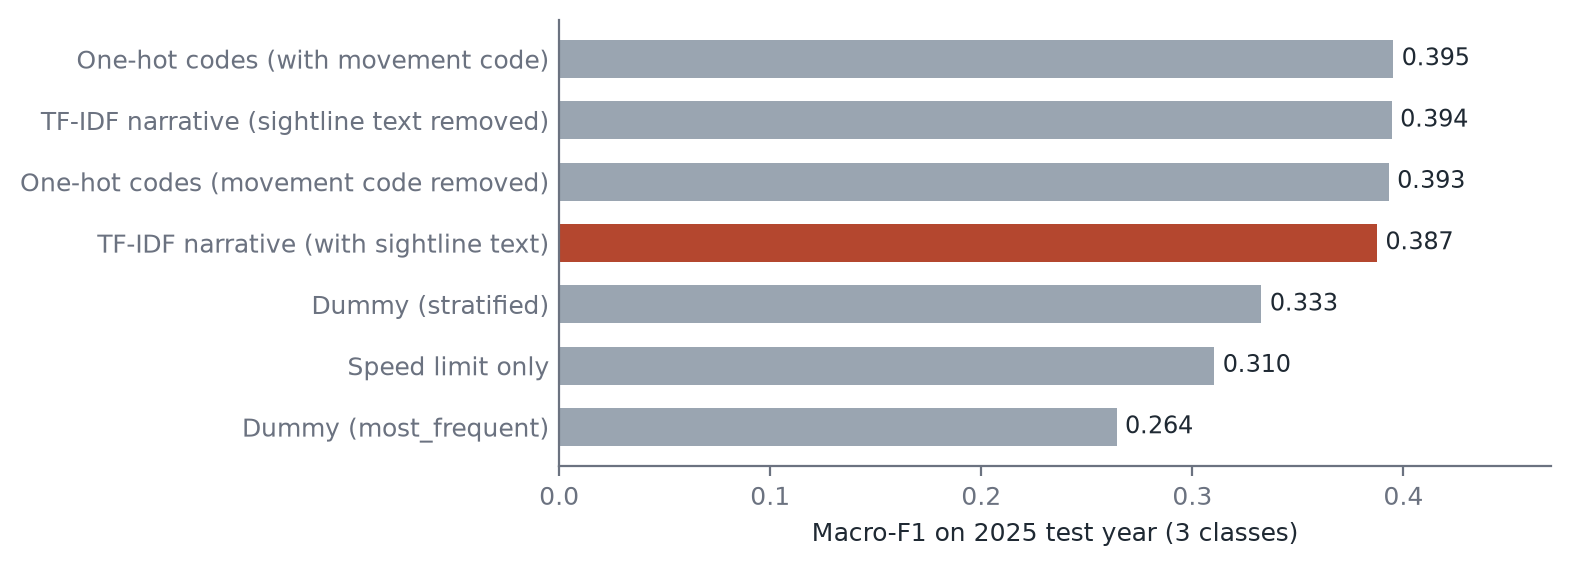
\includegraphics[width=14.5cm]{../results/figures/fig_models.png}\\[2pt]{\small\itshape Figure 1. Macro-F1 by feature set. The brief's model is highlighted.}\end{center}

Three readings. First, the model has real but limited skill: +0.055 macro-F1 over a stratified guess (95\% CI +0.040 to +0.069, paired bootstrap, 2,000 resamples), and well above speed limit alone (0.310). Second, TF-IDF text is not better than one-hot codes (difference -0.008, CI -0.013 to -0.002); it is slightly worse, as expected when 765 correlated phrases re-express 145 codes. Third, removing the sightline sentence does not reduce skill (with minus without: -0.007, CI -0.012 to -0.002).\par

\begin{center}\begin{minipage}{\textwidth}{\small\bfseries Table 3. Confusion matrix of the TF-IDF model on the test year.}\\[3pt]\small\setlength{\tabcolsep}{3pt}\begin{tabular}{@{}>{\raggedright\arraybackslash}p{0.313\textwidth}>{\raggedright\arraybackslash}p{0.202\textwidth}>{\raggedright\arraybackslash}p{0.202\textwidth}>{\raggedright\arraybackslash}p{0.202\textwidth}@{}}\toprule \textbf{Actual \textbackslash{} Predicted} & \textbf{Fatal} & \textbf{Serious} & \textbf{Slight} \\ \midrule 
Fatal & 122 & 39 & 53 \\
Serious & 541 & 467 & 2,866 \\
Slight & 401 & 528 & 6,868 \\ \bottomrule\end{tabular}\end{minipage}\end{center}

The model separates the extremes and not the middle: 2,866 of 3,874 serious injuries are called slight. The price of its fatal recall is 942 false fatal alarms for 122 true ones. The strongest phrases for the fatal class are ``aged 75'', ``pedestrian aged 75'', ``75'', ``going'', ``vehicle going ahead'', ``vehicle going'': age over 75, a vehicle going ahead (not turning or reversing) and heavy vehicles. The phrase ``masked parked'' ranks 564 of 765 for the fatal class (weight -0.065) and 271 for serious (+0.016): close to zero in both.\par

\section*{5. Does a blocked sightline raise severity?}

The hypothesis says sightline obstruction is a hidden predictor. The classifier says it adds no predictive skill. An odds ratio answers the narrower causal-flavoured question directly: among crossing pedestrians who were hit, are the masked ones more often killed or seriously injured (KSI)?\par

\begin{center}\begin{minipage}{\textwidth}{\small\bfseries Table 4. Crude 2 x 2 table. Odds ratio 1.04 (0.99 to 1.10).}\\[3pt]\small\setlength{\tabcolsep}{3pt}\begin{tabular}{@{}>{\raggedright\arraybackslash}p{0.423\textwidth}>{\raggedright\arraybackslash}p{0.166\textwidth}>{\raggedright\arraybackslash}p{0.166\textwidth}>{\raggedright\arraybackslash}p{0.166\textwidth}@{}}\toprule \textbf{} & \textbf{KSI} & \textbf{Slight} & \textbf{KSI rate} \\ \midrule 
Masked by parked or stationary vehicle & 2,520 & 4,841 & 34.2\% \\
Not masked & 16,136 & 32,334 & 33.3\% \\ \bottomrule\end{tabular}\end{minipage}\end{center}

\begin{center}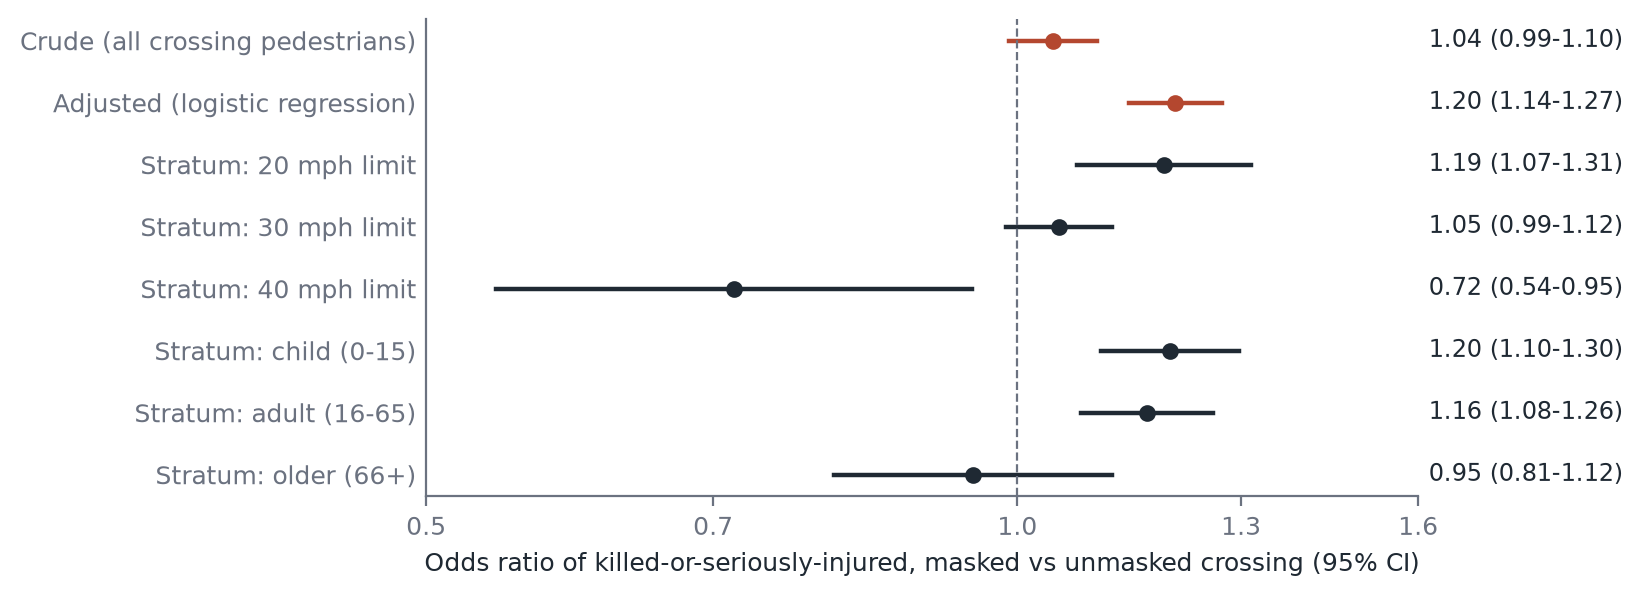
\includegraphics[width=14.5cm]{../results/figures/fig_forest.png}\\[2pt]{\small\itshape Figure 2. Odds ratio of KSI for masked against unmasked crossings: crude, adjusted, and within strata.}\end{center}

The crude ratio's interval includes 1. The adjusted ratio, from a logistic regression on 54,920 complete records, is 1.20 (1.14 to 1.27). The gap is confounding that runs against the effect: 48\% of masked casualties are children under 16 against 27\% of unmasked ones, and only 20\% happen in darkness against 31\%. Children (OR 0.90) and daylight carry lower severity, so the masked group looks safer than it is until those are held fixed.\par

\begin{center}\begin{minipage}{\textwidth}{\small\bfseries Table 5. Adjusted odds ratios for KSI (selected terms; full model in results/results.json).}\\[3pt]\small\setlength{\tabcolsep}{3pt}\begin{tabular}{@{}>{\raggedright\arraybackslash}p{0.552\textwidth}>{\raggedright\arraybackslash}p{0.368\textwidth}@{}}\toprule \textbf{Term (reference)} & \textbf{Odds ratio (95\% CI)} \\ \midrule 
Masked crossing (not masked) & 1.20 (1.14 to 1.27) \\
Darkness (daylight) & 1.47 (1.41 to 1.53) \\
20 mph limit (30 mph) & 0.85 (0.81 to 0.88) \\
40 mph limit (30 mph) & 1.82 (1.67 to 1.99) \\
60 mph limit (30 mph) & 3.48 (2.80 to 4.32) \\
Pedestrian aged 66+ (16 to 65) & 2.36 (2.25 to 2.49) \\
Child 0 to 15 (16 to 65) & 0.90 (0.86 to 0.94) \\
Heavy vehicle (car) & 1.74 (1.60 to 1.89) \\
On a crossing facility (elsewhere) & 0.89 (0.85 to 0.93) \\
Injury-based police reporting system & 1.34 (1.29 to 1.40) \\ \bottomrule\end{tabular}\end{minipage}\end{center}

Two cautions. The 40 mph stratum points the other way (0.72 (0.54 to 0.95)) on 227 masked casualties, so the effect is not uniform. And STATS19 records only collisions that injured someone: a masked crossing that ended in a near miss is not in the data, so these ratios describe severity given a collision, not the risk of a collision. The brief's near-miss escalation question cannot be answered from this source.\par

Verdict on the hypothesis: partly supported. Sightline obstruction is an independent severity factor of about 20\% higher odds, hidden in the crude data by who gets masked. It is not a strong enough signal to improve a classifier, and nothing here shows that text mining adds to the coded field.\par

\section*{6. STAMP analysis and the infrastructure constraint}

In STAMP an accident is a control problem: a safety constraint was not enforced by the control structure. The loss here is a pedestrian struck at a speed that kills or seriously injures; the hazard is a vehicle approaching a crossing faster than it can stop within the distance at which it can first see a pedestrian.\par

\begin{center}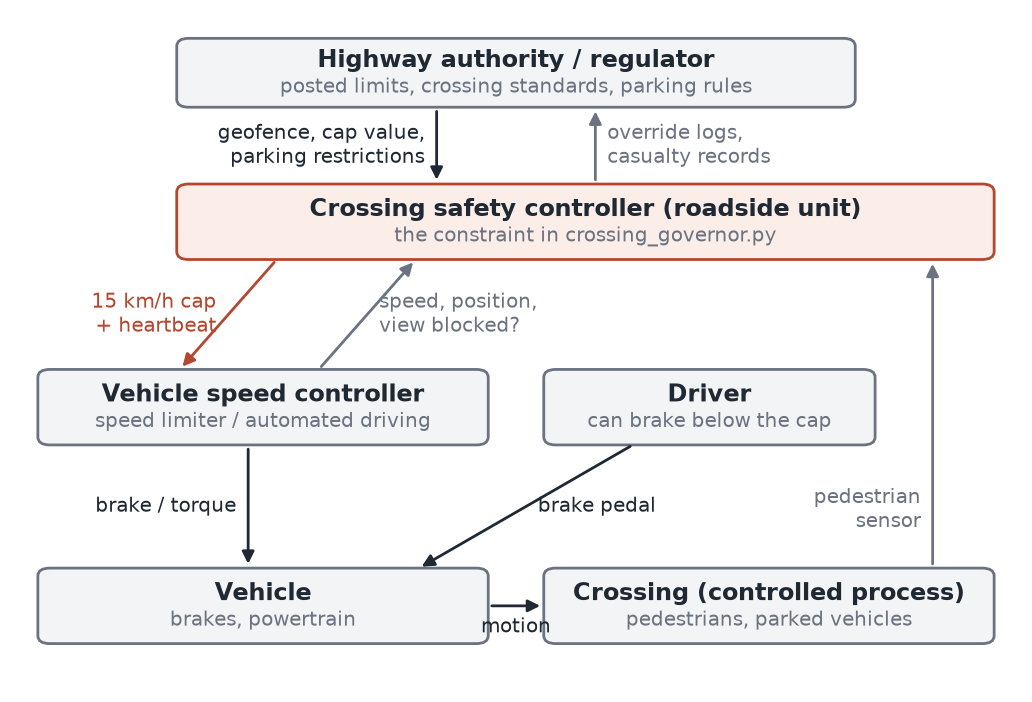
\includegraphics[width=12.5cm]{../results/figures/fig_control.png}\\[2pt]{\small\itshape Figure 3. Safety control structure for an instrumented crossing. Control actions point down, feedback up.}\end{center}

\subsection*{6.1 Is 15 km/h the right number?}

With a 1.0 s reaction time and 6.5 m/s\textsuperscript{2} emergency braking (assumptions, dry road), stopping distance is 5.5 m at 15 km/h, 15.1 m at 20 mph and 27.3 m at 30 mph. A pedestrian stepping out from behind a parked van is typically first visible within a few metres.\par

\begin{center}\begin{minipage}{\textwidth}{\small\bfseries Table 6. Impact speed by approach speed and the distance at which the pedestrian becomes visible.}\\[3pt]\small\setlength{\tabcolsep}{3pt}\begin{tabular}{@{}>{\raggedright\arraybackslash}p{0.221\textwidth}>{\raggedright\arraybackslash}p{0.175\textwidth}>{\raggedright\arraybackslash}p{0.175\textwidth}>{\raggedright\arraybackslash}p{0.175\textwidth}>{\raggedright\arraybackslash}p{0.175\textwidth}@{}}\toprule \textbf{First visible at} & \textbf{15 km/h (cap)} & \textbf{20 mph} & \textbf{30 mph} & \textbf{40 mph} \\ \midrule 
3 m & 15 km/h & 32 km/h & 48 km/h & 64 km/h \\
5 m & 9 km/h & 32 km/h & 48 km/h & 64 km/h \\
8 m & stops & 32 km/h & 48 km/h & 64 km/h \\
12 m & stops & 23 km/h & 48 km/h & 64 km/h \\
20 m & stops & stops & 35 km/h & 62 km/h \\
30 m & stops & stops & stops & 46 km/h \\ \bottomrule\end{tabular}\end{minipage}\end{center}

\begin{center}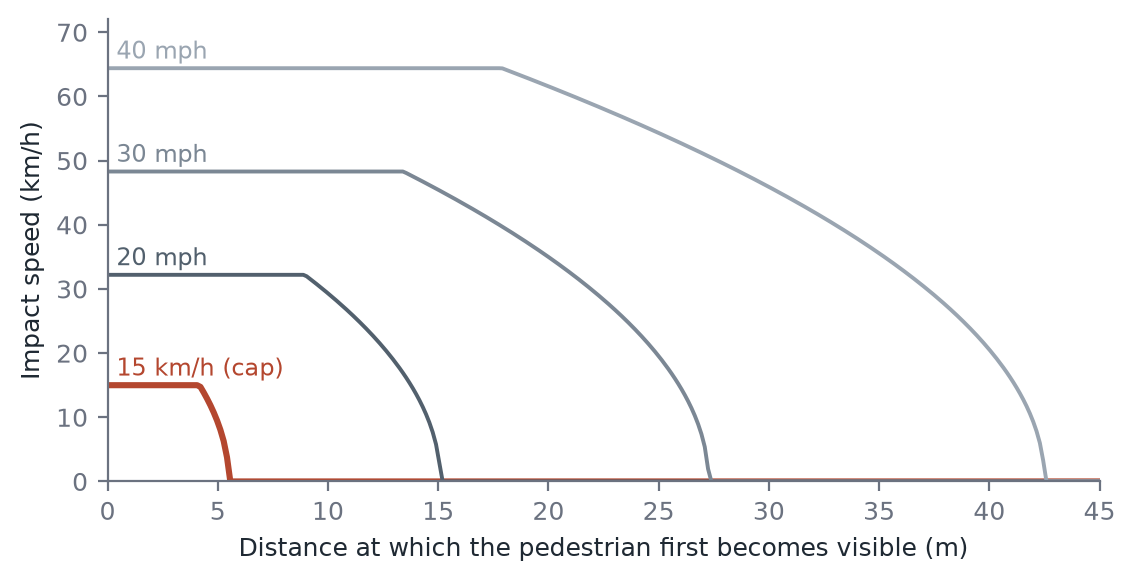
\includegraphics[width=14.5cm]{../results/figures/fig_impact.png}\\[2pt]{\small\itshape Figure 4. Impact speed against sight distance. The cap turns an 8 m emergence from a 48 km/h impact into a stop.}\end{center}

The cap does what it claims from about 5.5 m of sight distance upward, and below that the impact is at most 15 km/h. It does not guarantee a stop for a pedestrian who emerges inside 5 m; no speed above walking pace does. The data adds that the cap is a real override in most cases: 69\% of masked-crossing casualties were on 30 mph roads and 27\% on 20 mph roads.\par

\subsection*{6.2 Unsafe control actions}

The brief's rule covers one case: both signals healthy and true. STPA asks how the same control action becomes unsafe in the other cases. Each row below led to a requirement that the code enforces and a test checks.\par

\begin{center}\begin{minipage}{\textwidth}{\small\bfseries Table 7. Unsafe control actions for the 15 km/h override and the resulting requirements.}\\[3pt]\small\setlength{\tabcolsep}{3pt}\begin{tabular}{@{}>{\raggedright\arraybackslash}p{0.276\textwidth}>{\raggedright\arraybackslash}p{0.331\textwidth}>{\raggedright\arraybackslash}p{0.313\textwidth}@{}}\toprule \textbf{Unsafe control action} & \textbf{Why it is hazardous} & \textbf{Requirement added} \\ \midrule 
UCA-1. Cap not issued when a pedestrian is present and the view is blocked & Sensor fault, lost roadside link or unknown view state is read as ``no hazard''. & Missing or stale feedback is treated as hazard present: the cap applies (fail-safe). \\
UCA-2. Cap issued as an instant step change & Harsh braking from 30 mph invites a rear-end collision from a following vehicle. & Speed ramps to the cap at no more than 3.0 m/s\textsuperscript{2}. \\
UCA-3. Cap issued too late & Vehicle is already inside its stopping distance when the command arrives. & Approach zone long enough to finish the ramp: 15 m at 20 mph, 34 m at 30 mph, 59 m at 40 mph. \\
UCA-4. Cap released too soon & Sensor loses a pedestrian still hidden behind the parked vehicle; a second pedestrian follows. & Cap is held for 3 s after the hazard last appeared. \\
UCA-5. Cap issued outside the crossing zone & Nuisance overrides teach drivers to distrust or defeat the system. & No override outside the geofence; none when the view is clear. \\ \bottomrule\end{tabular}\end{minipage}\end{center}

The constraint is implemented in crossing\_governor.py as a deterministic rule, deliberately not a learned model: a classifier that misses 88\% of serious injuries cannot be the last line of defence. Twelve unit tests cover the brief's rule, each fail-safe path, the hold time, the ramp and the kinematics.\par

\subsection*{6.3 Coverage: where masked crossings actually happen}

\begin{center}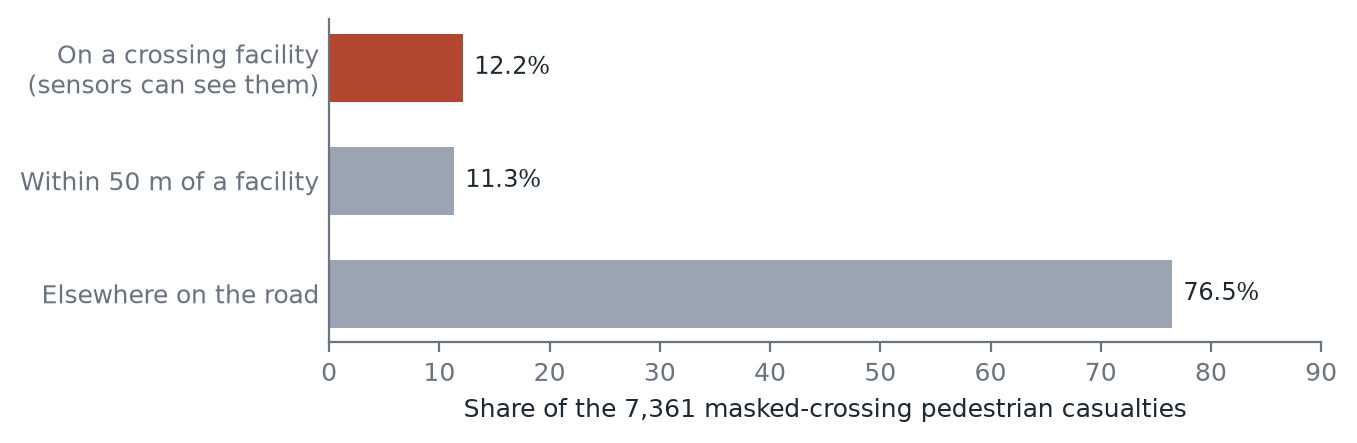
\includegraphics[width=14.5cm]{../results/figures/fig_coverage.png}\\[2pt]{\small\itshape Figure 5. Location of masked-crossing pedestrian casualties relative to crossing facilities.}\end{center}

An infrastructure-level constraint needs infrastructure. Of 7,361 masked-crossing casualties, 895 (12.2\%) were on a crossing facility or its zig-zag lines and a further 835 (11.3\%) within 50 m of one. For 66.4\% there was no crossing facility within 50 m at all. In severity terms the constraint as specified could have acted on 308 of 2,520 KSI casualties and 9 of 68 deaths. This is expected once stated: parking is already banned on zig-zag lines, so people are masked by parked vehicles mostly where there is no crossing.\par

The STAMP reading is that the constraint is placed at the wrong level of the control structure to control most of the hazard. Two changes follow. The same rule should also run on the vehicle, using its own perception of occluded kerbside space, so it works on any street. And the authority-level control, parking restrictions near informal crossing points such as school frontages, removes the occlusion instead of reacting to it.\par

\section*{7. Limitations}

\begin{itemize}\item The narrative is synthetic by construction. Real free-text narratives could carry details the codes lack; this study cannot say whether they do.
\item Severity is a proxy for escalation. No near-miss or timing data exists in the source.
\item Posted speed limit stands in for travel speed. Actual impact speeds are unknown.
\item The masked code is assigned by the reporting officer and may be under-recorded; ``unknown or other'' movement is 29\% of pedestrians.
\item Serious and slight are recorded differently by forces using injury-based systems (adjusted OR 1.34); it is a covariate in the regression but not in the SVM's target.
\item The stopping-distance figures rest on stated reaction and braking assumptions for a dry road. The constraint was tested in software only.
\item The coverage figures count casualties who could have been sensed, not casualties who would have been saved.
\end{itemize}

\section*{8. Reproducing this report}

\begin{quote}\small\ttfamily\raggedright .venv/bin/python analysis.py            \# merge, narratives, TF-IDF, SVM, odds ratios -> results/results.json\\ .venv/bin/python crossing\_governor.py   \# constraint kinematics -> results/constraint.json\\ .venv/bin/python -m pytest tests -q     \# 12 tests on the constraint\\ .venv/bin/python figures.py             \# results/figures/*.png\\ .venv/bin/python build\_report.py        \# report/*.docx and *.tex\end{quote}

\section*{Sources}

\begin{itemize}\item Department for Transport, Road Safety Data (STATS19): collision, vehicle and casualty tables, last five years, and the 2025 open dataset data guide. data.dft.gov.uk, Open Government Licence.
\item N. G. Leveson, Engineering a Safer World: Systems Thinking Applied to Safety. MIT Press, 2011.
\item N. G. Leveson and J. P. Thomas, STPA Handbook, 2018.
\end{itemize}

\end{document}